\section{线性规划简介}
\begin{frame}{\secname}
\begin{itemize}
    \item 线性规划是运筹学中研究最早,理论和算法比较成熟的一个重要分支,其应用十分广泛。
    \item 早在1939年,前苏联的数学家康托洛维奇(1975年诺贝尔经济学获得者)就提出了生产组织和管理中的线性规划模型。
    \item 20世纪40年代末,美国的Dantzig提出了求解一般线性规划的单纯形方法。Charnes对于线性规划的理论和应用也作出了突出的贡献。
    \item 目前可供计算大规模线性规划问题的计算机软件也较为成熟。因此,线性规划在工农业生产、商业活动、军事行动和科学研究的各个方面都得到了重要的应用。
\end{itemize}
 \end{frame}
 
 \subsection{线性规划模型}
\begin{frame}{\subsecname}
    %在了解线性规划的理论和应用前,必须先对线性规划模型有一个形象的映像。这一节将继续绪论中的讨论,首先介绍如何将真实问题转化为数学模型。下面通过两个示例(最优投资组合问题和投资决策问题)来介绍这一问题。
 \begin{example}[2-1:投资组合问题]
 一个投资者希望用一定数量的资金进行投资。他对10种不同的股票进行投资,并估计在1年内投资的收益。表2-1给出了每种股票的国别、风险类别(R为高风险,N为低风险)和期望投资收益率(ROI)。投资者确定了某些约束条件。为了分摊风险,他希望对每种股票的投资最多占总资金的30%。进一步,他希望资金的一半能够投资在北美的股票和最多 是高风险投资。这些资金应该怎样在各种股票中进行分配才能达到最大化的收益的目的呢?
 
 % Please add the following required packages to your document preamble:
% \usepackage[table,xcdraw]{xcolor}
% If you use beamer only pass "xcolor=table" option, i.e. \documentclass[xcolor=table]{beamer}
\begin{table}[]
\begin{tabular}{|c|c|c|c|c|}
\hline
\textbf{编号} & \textbf{描述} & \textbf{国别} & \textbf{风险类型} & \textbf{期望收益率} \\ \hline
\rowcolor[HTML]{FFFFFF} 
1           & 国库券         & 加拿大         & N             & 5              \\ \hline
\rowcolor[HTML]{FFFFFF} 
2           & 硬件          & 美国          & R             & 17             \\ \hline
\rowcolor[HTML]{FFFFFF} 
3           & 剧院          & 美国          & R             & 26             \\ \hline
\rowcolor[HTML]{FFFFFF} 
4           & 电信          & 美国          & R             & 12             \\ \hline
\rowcolor[HTML]{FFFFFF} 
5           & 酿酒          & 英国          & N             & 8              \\ \hline
\rowcolor[HTML]{FFFFFF} 
6           & 高速公路        & 法国          & N             & 9              \\ \hline
\rowcolor[HTML]{FFFFFF} 
7           & 汽车          & 德国          & N             & 7              \\ \hline
\rowcolor[HTML]{FFFFFF} 
8           & 银行          & 卢森堡         & N             & 6              \\ \hline
\rowcolor[HTML]{FFFFFF} 
9           & 软件          & 印度          & R             & 31             \\ \hline
\rowcolor[HTML]{FFFFFF} 
10          & 电子          & 日本          & R             & 21             \\ \hline
\end{tabular}
\end{table}
 \end{example}   
\end{frame}

\begin{frame}{\secname}
    解:为了构建数学模型,首先要确定问题的解中包含的决策变量:在当前的案例中,希望知道整个投资中每种股票的投资数量。因此,定义决策变量 表示股票 在投资资金中所占的比例。这也就意味着所有变量都必须是一个在0和1之间的分数(其中1代表整个资金的100\%)。事实上,每个变量都有一个最大值约束,即投资者期望的投资每种股票最多占整个资金的30\%。以下约束条件建立了所有变量的边界:
$$
0 \le x_i \le \frac{1}{3}, \quad i=1,2,\dots, 10.
$$
将$w_i$ 作为股票$i$的期望ROI,在这里表示:
$$
w=(5,17,26,12,8,9,7,6,31,21)
$$
投资者希望将所有的资金都进行投资,也就是说不同股票的分数之和必须为100%。这可以表达为以下等式约束:
$$
\sum_{i=1}^{10} x_i =1
$$
\end{frame}

\begin{frame}{\subsecname}
现在仍然需要两个约束条件来表达投资者的特殊要求。至多1/3的资金是高风险股票,即投资到这个类型股票的资金之和不能超过整个资金的1/3:
$$
x_2+x_3+x_4+x_9+x_{10} \le \frac{1}{3}
$$
投资者同样坚持对北美的股票的投资最少50%:
$$
x_1+x_2+x_3+x_4 \ge \frac{1}{2}
$$
这两个约束条件为不等式约束。
    投资者的目标是最大化所有股票投资的收益,也就是说最大化下面的表达式:
$$
\sum_{i=1}^{10} w_ix_i
$$
这就是数学模型的目标函数。
\end{frame}

\begin{frame}{\subsecname}
\begin{block}{线性规划模型}
可以得到以下整个数学模型的表达式:
\begin{alignat}{2}
&&\min\quad   \sum_{i=1}^{10} w_i x_i \\
\mbox{s.t.}\quad
\left\{
\begin{array}{cc}
     & \sum_{i=1}^{10} x_i =1 \\
     & x_2+x_3+x_4+x_9+x_{10} \le \frac{1}{3}\\
     & x_1+x_2+x_3+x_4 \ge \frac{1}{2} \\
     & x_i \ge 0, \quad i=1,2,\cd, 10.
\end{array}
\right.
\end{alignat}
\end{block}
\end{frame}

\begin{frame}{\subsecname}
通过对这个问题的解读,已经将以上的模型建立起来了。其中,“maximize”表示最大化。S.t.是英文“subject to”的缩写,“使得”的意思。下面来回忆一下整个建模过程和线性规划的一些特点:
\begin{itemize}
    \item 全面了解问题。
     \item 描述目标。
\item 描述约束条件。
\item 定义决策变量。
\item 用决策变量写出目标和约束条件。
\end{itemize}
以上问题就是线性规划模型或者线性规划。正如前面所述,该问题有目标和约束条件,这是所有线性规划所共有的特点。并且它的目标函数和约束条件都是关于决策变量的线性函数。线性函数是指函数中的每个变量都是分离的并且幂次为1。在刚才的模型中,目标函数是线性函数,因为所有的决策变量都是分离的,并且都是一次幂。约束条件的左边都是线性函数,因此称此问题为线性规划。

线性规划有3个基本的假设:比例性、可加性和可分性。比例性是指目标函数值和约束条件所对应的资源值与决策变量值成比例。可加性是指目标函数的值和使用资源总量分别可以通过汇总所有的决策变量对目标函数的贡献和各个决策变量使用资源数量而得到。可分性是指决策变量是连续的。非负条件和可分性假设意味着决策变量可以是大于或者等于零的一切数值。

\end{frame}

\begin{frame}{\subsecname}

      \begin{example}
      某公司有100万的资金可供投资。该公司有六个可选的投资项目,其各自的数据如表2-2所示:
% Please add the following required packages to your document preamble:
% \usepackage[table,xcdraw]{xcolor}
% If you use beamer only pass "xcolor=table" option, i.e. \documentclass[xcolor=table]{beamer}
\begin{table}[]
\begin{tabular}{|c|c|c|c|c|}
\hline
\textbf{投资项目} & \textbf{风险(\%)} & \textbf{红利(\%)} & \textbf{增长率(\%)} & \textbf{信用度} \\ \hline
\rowcolor[HTML]{FFFFFF} 
1             & 18             & 4              & 22              & 4            \\ \hline
\rowcolor[HTML]{FFFFFF} 
2             & 6              & 5              & 7               & 10           \\ \hline
\rowcolor[HTML]{FFFFFF} 
3             & 10             & 9              & 12              & 2            \\ \hline
\rowcolor[HTML]{FFFFFF} 
4             & 4              & 7              & 8               & 10           \\ \hline
\rowcolor[HTML]{FFFFFF} 
5             & 12             & 6              & 15              & 4            \\ \hline
\rowcolor[HTML]{FFFFFF} 
6             & 8              & 8              & 8               & 6            \\ \hline
\end{tabular}
\end{table}
      该公司想达到的目标为:投资风险最小,每年的红利至少为6.5万元,最低平均增长率为12\%,最低平均信用度为7。
      \end{example}

\end{frame}

\begin{frame}{\subsecname}
    解:首先面对这一问题,要抓住决策变量、目标以及约束条件。
    \begin{itemize}
        \item \red{决策变量}:本问题的决策变量是在每种投资项目上的投资额。设$X_i$为项目i的投资额。
        \item \red{目标函数}:本问题要求总投资最小,即:
        $$
        \min \quad z=0.18x_1+0.06x_2+0.1x_3+0.04x_4+0.12x_5+0.08x_6
        $$
        \item \red{约束条件}:本问题共有5个约束条件。这些约束可以表示为:
        \begin{itemize}
            \item 各项目投资总额为100万: \\ $x_1+x_2+x_3+x_4+x_5+x_6=100$.
            \item 每年的红利至少为6.5万:\\
            $0.04x_1+0.05x_2+0.09x_3+0.07x_4+0.06x_5+0.08x_6 \ge 6.5$.
            \item 最低平均增长率为12\%:\\
        $0.22x_1+0.07x_2+0.12x_3+0.08x_4=0.15x_5+0.08x_6 \ge 100\times 12\%$
           \item 最低平均信用度为7: \\
           $4x_1+10x_2+2x_3+10x_4+4x_5+6x_6 \ge 7 \times 100$
           \item 非负约束:\\
           $x_1, x_2,x_3,x_4,x_5,x_6 \ge 0$
        \end{itemize}
    \end{itemize}
\end{frame}

\begin{frame}{\subsecname}
  
    \begin{block}{数学模型}  
    于是得到以下的线性规划模型:
\begin{alignat}{2}
\min\quad  z=0.18x_1+0.06x_2+0.1x_3+0.04x_4+0.12x_5+0.08x_6 \nonumber\\
\mbox{s.t.}\quad
\left\{
\begin{array}{cc}\nonumber
     & x_1+x_2+x_3+x_4+x_5+x_6=100 \\
     & 0.04x_1+0.05x_2+0.09x_3+0.07x_4+0.06x_5+0.08x_6 \ge 6.5\\
     & 0.22x_1+0.07x_2+0.12x_3+0.08x_4=0.15x_5+0.08x_6 \ge 100\times 12\% \\
     & 4x_1+10x_2+2x_3+10x_4+4x_5+6x_6 \ge 7 \times 100 \\
     & x_i \ge 0, \quad i=1,2,\cd, 6.
\end{array}
\right.
\end{alignat}
\end{block}

\begin{alertblock}{注:}
  这是一个典型的成本(或者风险)最小化问题。模型的意义是在给定的限制条件下,求使得目标函数达到最小时的每个项目投资额。可以看到,以上问题是线性规划模型。该问题有目标和约束条件,其目标函数和约束条件都是决策变量的线性函数,也满足线性规划的3个基本假设。
\end{alertblock}

\end{frame}

\subsection{图解法}
\begin{frame}{\subsecname}
    对模型中只含有2个变量的线性规划问题,可以通过在平面上作图的方法求解。通过图解法,可以对线性规划问题及其求解过程有一个直观的认识,便于建立N维空间中线性规划问题的概念,同时帮助读者更好地理解求解一般线性规划问题的单纯形法的思路。
\end{frame}

\subsubsection{线性规划问题图解法的步骤}
\begin{frame}{\subsubsecname}
    为了便于理解,下面将通过抽象出来的数学规划模型来具体说明线性规划问题图解法的步骤,以便理解。
    \begin{example}[例2-3] 
    考虑只有两个变量的线性规划问题,用图解法解答:
    \begin{alignat}{2}
\min\quad  z=x_1+3x_2 \nonumber\\
\mbox{s.t.}\quad
\left\{
\begin{array}{cc}\nonumber
     & x_1+x_2 \le 6 \\
     & 2x_1-x_2 \ge 0\\
     & x_2 \le 3\\
     & x_i \ge 0, \quad i=1,2.
\end{array}
\right.
\end{alignat}
    \end{example}
\end{frame}

\begin{frame}{\subsubsecname}
\begin{itemize}
    \item 在平面上建立直角坐标系
    \item 根据图示约束条件,找出可行域
     \item 图示目标函数
     \item 寻找最优解
\end{itemize}
    最优解的目标函数值为:
    $$
    z=x_1+3x_2=3+3\times 3 = 12
    $$
\end{frame}

\begin{frame}{\subsubsecname}
\centering
       \begin{tikzpicture}
    % the axis environment 
    \begin{axis}[axis x line=middle,
                 axis y line=middle,
                 xmin=-1,xmax=6,
                 ymin=-1,ymax=6,
                 ylabel=$x_2$,
                 xlabel=$x_1$]
        \addplot[elegant,red,domain=0:12]{2*x};
        \addplot[elegant,green,domain=0:10]{3};
        \addplot[elegant,orange,domain=0:6]{6-x};
       \addplot[elegant,black,domain=0:6]{-1/3*x+4};
    \end{axis}
\end{tikzpicture}

\end{frame}

\subsubsection{线性规划解的情况}
\begin{frame}{\subsubsecname}
  \begin{itemize}
    \item 有唯一的最优解
    \item  有无穷多最优解
    \item 无界解
    \item  无解,或无可行解
\end{itemize}  
\begin{figure}\label{fig:ch2-2}
  \centering
  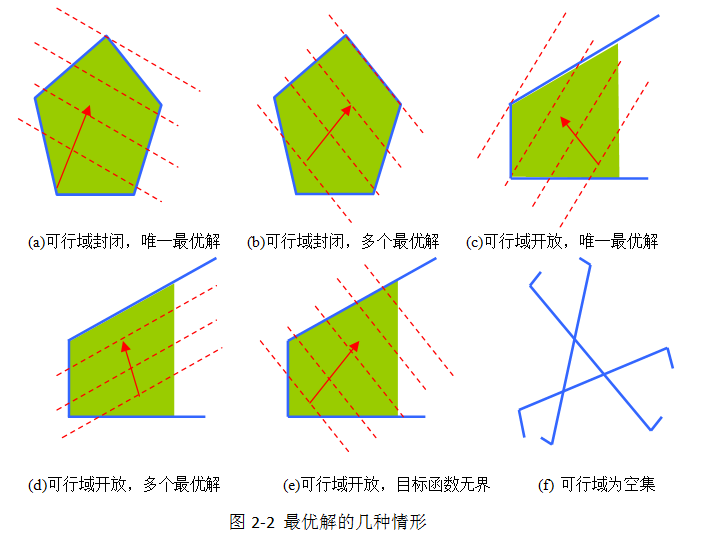
\includegraphics[width=4 in,height=2.5 in]{pic/2_2.png}
  \caption{最优解的几种情形}
\end{figure}
\end{frame}

\subsubsection{线性规划问题的标准形式}
\begin{frame}{\subsubsecname}
 由于目标函数和约束条件在内容与形式上的差别,导致线性规划问题表达多种多样,为了便于讨论线性规划问题的求解方法和解的性质,需要规定线性规划问题的标准形式。如果一个线性规划问题满足以下条件,就称为标准形式的线性规划问题:
 \begin{enumerate}
        \item 求目标函数的最大值;
        \item 所有变量均要求取非负值;
        \item 所有的约束条件(变量非负约束除外)必须为等式;
        \item 约束条件右端常数项$b_i$全为非负值。
\end{enumerate}
\end{frame}

\begin{frame}{\subsubsecname}
    \begin{alignat}{2}
\max \quad  z=\sum_{j=1}^n c_jx_j \nonumber\\
\mbox{s.t.}\quad
\left\{
\begin{array}{cc}\nonumber
     & \sum_{j=1}^n a_{i,j}x_j=b_i \quad i=1,2,\cd, m\\
     & x_j \ge 0, \quad j=1,2, \cd, m.
\end{array}
\right.
\end{alignat}
标准形式的矩阵表达式如下:
 \begin{alignat}{2}
\max \quad  z=c^Tx \nonumber\\
\mbox{s.t.}\quad
\left\{
\begin{array}{cc}\nonumber
     & \vA X = b\\
     & x_j \ge 0, \quad j=1,2, \cd, m.
\end{array}
\right.
\end{alignat}
其中,
$$
\begin{gathered}
   c=
    \begin{bmatrix}
    c_1 \\c_2 \\ \vdots \\c_n
    \end{bmatrix}
    \quad
  X= \begin{bmatrix}
    x_1 \\x_2 \\ \vdots \\x_n
    \end{bmatrix}
    \quad
  b= \begin{bmatrix}
    b_1 \\b_2 \\ \vdots \\x_m
    \end{bmatrix}
    \vA=
    \begin{bmatrix}
    a_{11}&a_{12}&\cd &a_{1n}\\
    a_{21}&a_{22}&\cd &a_{2n}\\
    \cd &\cd& \cd &\cd\\
    a_{m1}&a_{m2}&\cd &a_{mn}
    \end{bmatrix}
\end{gathered}
$$
\end{frame}

\subsection{线性规划的基本概念}
\begin{frame}{\subsecname}
    对于各种非标准形式的线性规划问题,总可以通过以下的变换,将其转化为标准形式。
\begin{itemize}
    \item[(1)] 极小化目标函数的问题:
\item[(2)] 约束条件不为等式的问题:
\item[(3)] 变量无符号限制的问题:
\item[(4)] 变量小于等于零的问题:
\end{itemize}
\end{frame}

\subsubsection{线性规划问题的解}
\begin{frame}{\subsubsecname}
    在图解法中,已经比较直观地讨论了线性规划问题的可行解和最优解等概念,但图解法无法解决三个及其三个变量以上的线性规划问题,为了用代数方法求得可行域的极点,还需要引入以下一些有关线性规划可行域和解的概念。
\begin{definition}[超平面]
在n维空间中,满足条件:
$
a_{i1}x_1+a_{i2}x_2+ \cd +a_{in}x_n=b_i
$
的点集$X=(x_1,x_2,\cd,x_n)^T$ 称为一个\red{超平面}。
\end{definition}
\begin{definition}[半空间]
在n维空间中,满足条件:
$
a_{i1}x_1+a_{i2}x_2+ \cd +a_{in}x_n \le (或者 \ge ) b_i
$
的点集$X=(x_1,x_2,\cd,x_n)^T$ 称为一个\red{半空间}。
\end{definition}
\begin{definition}[多面体]
有限个半空间的交集,即同时满足以下条件的非空点集:
$$
a_{i1}x_1+a_{i2}x_2+ \cd +a_{in}x_n\le (或 \ge ) b_i
,\quad i=1,2,\cd, m 
$$
的点集$X=(x_1,x_2,\cd,x_n)^T$ 称为一个\red{多面体}。
\end{definition}
\end{frame}

\begin{frame}{\subsubsecname}

\begin{definition}[线性规划的基]
对于线性规划的约束条件
$$
\vA X=b
$$
$$
X \ge 0
$$
其中$\vA$为$m\times n$的矩阵,$n>m$,秩$\vA=m$,$b$为$ m \times 1$向量。设$\vB$是$\vA$矩阵中的一个非奇异的$m\times m$子矩阵,则称$\vB$为线性规划的一个\red{基}。
\end{definition}

\begin{definition}[基解、基可行解和可行基]
线性规划的解:
$$
X=\begin{bmatrix}
X_B \\ X_N
\end{bmatrix}
=\begin{bmatrix}
B^{-1}b \\ 0
\end{bmatrix}
$$
称为线性规划与基$\vB$对应的基解。
\end{definition}
\end{frame}

\section{线性规划的计算机求解}
\subsection{用Excel“规划求解”功能求解线性规划}
\begin{frame}{\subsecname}
\begin{itemize}
    \item 在Excel电子表格中建立线性规划模型
    \item 利用Excel“规划求解”功能求解线性规划问题
    \begin{itemize}
        \item “Set Target”(设置目标单元格):在这一栏中,输入表示目标函数值的单元格地址“B10”(也可以直接单击B10单元格)。
        \item “Equal to”(等于):选中“min”;
        \item 在“By changing cells:”中输入:B4:G4表示决策变量的位置。
        \item 在“subject to the constraints”一栏中通过“Add”添加约束条件。
        (5)单击“Options”按钮,在弹出的“Solver Options”对话框中,设置求解运算中的有关参数。本问题需要选择“Assume Linear Model”和“Assume Non-Negative”。这是采用线性模型和假定非负的复选框,单击确定;
\item 单击左上角的“Solve”按钮,则开始进行规划求解。
\item 在弹出的“Solver Results”对话框中(注意:当模型没有可行解或者目标值为无穷的时候,规划求解结果的内容将不同),选中“keep Solver Solution”,保存结果,单击“OK”。
    \end{itemize}
\end{itemize}
\end{frame}

\subsubsection{用LINDO/LINGO求解线性规划问题}
\begin{frame}{用LINDO求解线性规划问题}
    安装好LINDO软件包以后,点击执行文件。此时会弹出LINDO软件的空白对话框。在空白对话框中就可以直接书写命令了。\\
下面给出其结果的一般解释:
\begin{itemize}
    \item “LP OPTIMUM FOUND AT STEP 3”表示LINDO 在(用单纯形法)3次迭代或旋转后得到最优解。
    \item “OBJECTIVE FUNCTION VALUE 1) 8.25”表示最优目标值为8.25。
“VALUE”给出最优解中各变量的值。
\end{itemize}
要得到以上结果,必须遵循以下简单的软件规则:
\begin{itemize}
    \item (1) 目标函数及各约束条件之间一定要有“Subject to (ST) ”分开。
\item (2) 变量名不能超过8个字符。
\item (3) 变量与其系数间可以有空格,单不能有任何运算符号(如乘号“*”等)。
\item (4) 要输入<=或>=约束,相应以<或>代替即可。
\item (5) 一般LINDO 中不能接受括号“()“和逗号“,“,例:400(X1+X2) 需写成400X1+400X2;10,000 需写成10000。
\item (6) 表达式应当已经简化过。不能出现 2 X1+3 X2-4 X1,而应写成-2X1+3 X2。
\end{itemize}

\end{frame}

\begin{frame}{LINGO软件求解线性规划}
    LINGO是求解优化问题的一个专业工具软件,它包含了内置的建模语言,容许用户以简单直观的方式描述较大规模的优化模型,对于模型中所需要的数据可以以一定的形式保存在独立的文件中,读取也很方便快捷。
    
    一般来说,在LINGO中建立优化模型都是由四个部分组成,也即是:集合段,数据段,初始段以及目标与约束段。每个模型都是由model语句开始,由end语句结束。
    
\end{frame}
